\section{Франкенвордические неформологизмы}
\begin{epigraph}
        Скажем "Гоп", когда ляжем в гроб.\\
        Немного чёрного юмора, 18 сентября 2016 % куда уж без него
\end{epigraph}
Ужачно = удачно + ужасно --- ужасно удачно\\

\emph{Аналогично:} уржачно\\

Бабаня --- \emph{ну тут всё ясно, а вот следующее --- это ещё одно слово с 2-мя буквами ё:} Тётёля

\begin{figure}[ht!]
    \centering
    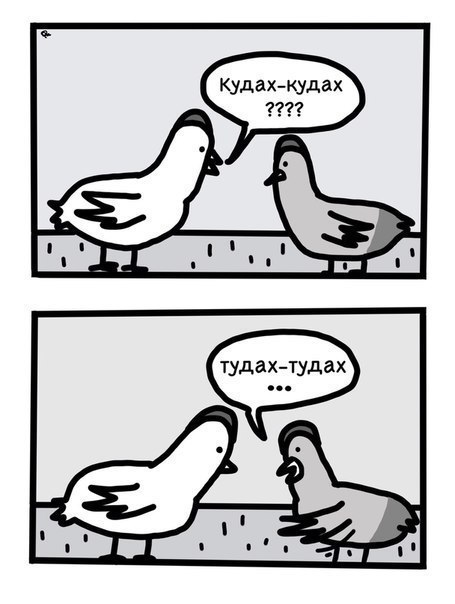
\includegraphics[width=0.6\textwidth]{tudakh}
    \caption{Alice, stop using drugs!}
\end{figure}

Идея: написать маленький рассказ из набора фраз на одну букву.\\
Главное условие: не меньше 3-х слов подряд должны быть на одну букву.

\subsection{Как заставить всех людей строить странные предложения и не стать психом}
\emph{Собственно весь "рассказ" --- это просто диалог двух обычных квазисреднестатистических людей, что является реализацией ещё одной идеи по попутному написанию литературных творений в любой наперёд заданной форме.}

\begin{flushleft}\parskip1em
    \emph{Я прочувствовал дух однобуквенного высказывания:}
    Василий Васильевич Васильев всё время валял вал\\
    --- Всё валяешь вал?\\
    --- Валяю вал\\
    --- Вандал! Варварство! Ватман!\\
    --- Ватман?\\
    --- Вероломство!\\
    Вдохновленный вандал всё валял, валял... Великолепно валял вал.

    --- Вы вдохновенно ввалились в...\\
    --- ...высказывание?\\
    --- Возможно.\\
    --- Вероятно вы верно вещаете.\\
    --- Ворчанием воздержитесь воздавать возведённое великолепие.

    \emph{"Великолепное ворчание всё время воздаёт величественную возню!"}
    \vspace*{-1em}\begin{flushright}
        Великий Воитель
    \end{flushright}

    \emph{Вычурно вы выводите все ваши высказывания, владыка!}

    \emph{Владею, верую, воздаю!}

    \emph{Вмиг вмешиваете вменяемость в виртуально вывитую вещь.}

    \emph{Виртуозно и вычурно вывернул!}

    \emph{Наитивно навыком научились науськивать наши недра неких надумок.}

    \emph{Адски азартно аплодирую!}

    \emph{Да, довольно дельно думать научился на наших беседах без больших затрат за звено времени возымевшимся в своём распоряжении.}

    \emph{Дык, договорились делать данный диалог в выбранной высказывательной форме.}

    \emph{Хорошо хоть хочу делать данный диалог.}

    \emph{Этот эдакий энтузиазм иссякнуть или исчезнуть вполне внезапно возымеет --- надо наибольшее напряжение проявить при проектировании фантазируемых фурорных фраз.}

    \emph{Очень Ожегова освежить снова следует сейчас. Коль когда костноязычно говоришь --- голова гудит}

    По простецкой по причине\\
    Коль когда костноязычишь\\
    Говоришь гундёж гремучий\\
    Ты теперь тут получай

    \vskip1em

    \emph{[полубелый стих]}\\
    Трудно трутню трюизмами\\
    Изысканные измышления изваять.\\
    Посему повелеваем вам\\
    Книжки купленны читать

    Загнуть заросли загубленных\\
    Мыслей мешает мука моя:\\
    Придумки повес пришлашённых\\
    Расхоже расценила моя семья

    Туманно тучи толпятся в ночи\\
    Ты тоже теперь его не ищи\\
    Закинул зелёную зарисовку подальше\\
    Не будет не будет теперь всё иначе\\

    \vskip1em

    \emph{\anttf{на этом месте мы раскрыли причину того, почему в песнях такая муть встречается. 
    Мы раскрыли их зловещий план! --- Теперь мы гребём бабло! и выбрали девиз для мёртвой сосны}}

    \emph{\anttf{Тут просто открыл словарь и читаю слова на одной стр:}}\\
    \emph{Дубильщик дубасит дрянной дубиной дрябоый дуализм дублируя дублоны дружинника...}

    \emph{Пошёл поток прекрасных новых неформальных неологизмов!}

    \emph{"Фокусник Фёдор фелонит"}

    \emph{феерично фыркнул фуникулёрщик}
    
    \emph{Пришла пора продолжать доделывать договорённый диалог ---\\
        Сегодня солирую самостоятельно\\
        Хорошо (бы) хоть хватило сил сочинять семь строк, но на ночь каждого календарного кончающегося дня\\
        Здорово задействовать бы большинство букв азбучного англо-русского алфавита\\
        Фонетический фокус фолиант поможет проделать при правильном пользовании\\
        Царапать ценные цепляющие фразы фантазия форы несколько немного не даёт\\
        Изрыл и изьял из памяти последнего полугода около 11 осмысленных различных разговорных ребусов такой требуемой тематики\\
        Может мысли методом, по примеру поэта серебряного столетия Сашки Блока, бороздами блочить будем?\\
        Переберём поэта по полочкам\\
        Пожалуй пора прекращать поток пробившихся присказок - пока предостаточно для данного дня}
    \emph{вон валяется величественный властитель\\
        невежественно-наивный носок\\
        никогда никому ничего не нужно\\
        вперёд! винтажный воитель\\
        бюджетная безграничная бездна}
    \emph{не надо, не мутузь муза меня ---\\
        пожайлуста, по-мутузь просто коня}
    \emph{Йспользуя редкие буквы в рубрике наркомании:\\
    Йошкар-олинский йог йодль исполнял и йодом Йорк исписан на спине товарища}
    \emph{ну не надо спешить со словами-то}
    \emph{--- Йошкар-ола, Йошкар-ола. Йа Йонаго.\\
        --- Йонго, Йето Йошка-ола. Йокосука Йоегер у Йома.\\
        пример плохого диалога у радистов}
    \emph{Блеяние баранов-бездельников барабаны перебивало пока проводился парад}
    \emph{Бесчиленное большенство барабанно-банановых баранов бездельников безудержно бле(е/я)ли}
    \emph{offtop: Банано-барановый пудинг к Куйрам Байрану - идея для десерта}
    \emph{Шипящий шелест штор ночью ни на секунду спать спокойно возможности взять не возымел}
    \emph{Конфликтный каратист казахской коренастости купит килограмм конфет}
    \emph{Важные воры воровали восхитительных ворон. Вдруг в воздухе воцарился вакуум.
    Всё вблизи вальсировало в вальсе Вавилона. Вдали вдруг возник вожатый. Всё время важничал.
    Велосипед ведь вензельный вероломно вертели.\\
    Вердикт — виновен.}
    \emph{Высокопарно вывели вашу надумку натруженному народу}
    \emph{Отрицать отточенное образование никогда не нужно}
    \emph{начинаем нарабатывать наркоманско-дармоедовские диалоги ---\\
    историческая история о историческо-идеалитическо-идеализированных историях\\
    комбинированный кроссворд круговыми кардиограммами\\
    Кто? Кто?! Кто копать картошку кинулся?}
    \emph{Франкфуртские философы французских фазанов, фамильярно фанаберившихся, феерично фехтовали фонтанами фитюлек.\\
    Финские физики-флибустьеры флегматично фыркали, фривольно фантазируя фрегат форшмака.\\
    - Фьють! - фырчала фольклористка-фотомодель фольгой фортепиано фартово фортелируя 
        [фортель - ловкая проделка. неожиданная выходка]\\
    Фееричный форсаж фантазии —- фамильная черта четы Чебышевых.\\
    Колонка клокотала колоколами будильника будя баллотировавшихся бакалавров —- будущих банкротов, безмятежно беллетристической белибердой беседы бичевавших.\\
    Cлаженно скатившись со склона скалы Славик со Светой сгребли снега с лихвой.}
    \emph{Ну и напоследок немного наркомании:\\
    freelancer —- фиолетовая фигня, феерично фонтанирующая фривольными фразами.\\
    Сегодня семь сантисказок}
    \emph{-— Пппеперонни, - представился перед постовым подвыпивший преступник.\\
    Тролли трескали треску, трепыхая требухой.\\
    Художник хутора Хорьков хотел хвастаться хиджабом, хлебнув хорошо хмельного "хлеба"\\
    Олег остекленело осмотрел Осётрова, основательно осевшего оземь от обрушившейся, оторвавшейся оси.\\
    -— Убирайся! - устал упрашивать убийца.\\
    Парикмахер Паша придумал пасхалку припрятать при прочтении повести писателя По.\\
    Сегодня снова семь сказок, считая сею}
    \emph{Стих о парне, который на ночь читал теорию поля и начал засыпать:\\
    Ландау-Лившица листая\\
    Лотков легонько лёг лежать.\\
    Лицо любимой лобызая ---\\
    Лекало ложкой ли ломать?}

    \emph{Селёдка, соль (и) семечки' ---\\
    Сегодня снова снедь сия\\
    С Сенекой, Сатром, Сальери'\\
    С собою с сумкой (я) снесла.}

    \emph{Писатель поэту повесть подарил,\\
    Поэт писателю поэму посвятил.\\
    Писатель поэту посуду перебил,\\
    Поэт писателя почку продавать переубедил.}
    \emph{Прекращаем придумывать представленную придурь пока погода позволяет.}
    \end{flushleft}
% немного рекламы
\begin{figure}[ht!]
    \centering
    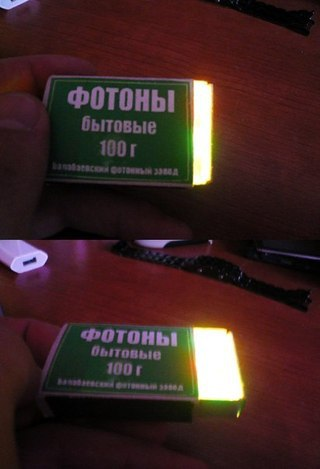
\includegraphics[width=\textwidth]{fot}
    \caption{Свежие фотоны у вас меньше чем за 8 минут!}
\end{figure}

\subsection{Словесно-свойственный shashlik}
Берём слово и набираем близкие по смыслу слова или действия совершаемые данным объектов, но на другую букву.


конь — пегас — возило — летало — кусало — ржало


вот очень краткое: заменяло


барашка --- шерстилось --- мекало --- жарилось --- продавалось --- елость
\vskip4em

\framebox[0.9\textwidth][c]{
    Здесь могла быть ваша реклама, но нет!
}
